\documentclass[../diagrams.tex]{subfiles}

\begin{document}
\label{diagrams:activity_diagrams}

\subsubsection{Uzyskanie sesji}

Proces opisuje prośbę klienta o ustanowienie dla niego sesji. Sesja może już istnieć albo zostać utworzona.

\begin{figure}[!h]
	
	\centering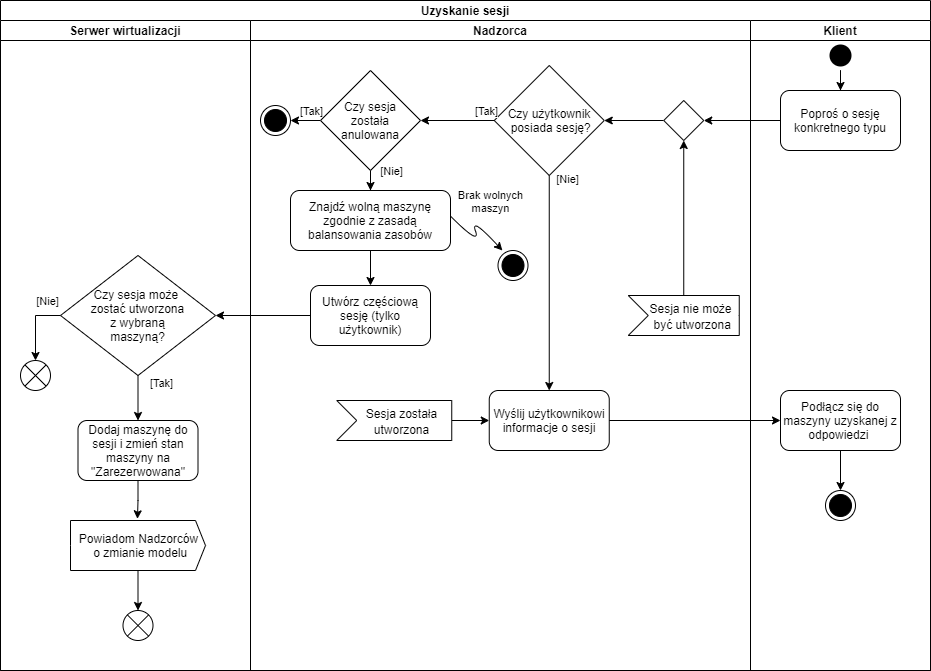
\includegraphics[width=\textwidth]{activity_diagrams/uzyskanie_sesji.png}
	
	\vskip-1.5ex
	
	\caption{Diagram aktywności dla uzyskania sesji}
	\label{start_session}
\end{figure}

W przypadku istniejącej już sesji nadzorca przekazuje od razu cały gotowy obiekt sesji.
W przeciwnym razie nadzorca zaglądając do modelu systemu znajduje pewną wolna maszynę(dla konkretnego stanu modelu za każdym razem musi być wybrana ta sama maszyny - powtarzalność)
i informuje serwer wirtualizacji o prośbie utworzenia sesji.
Gdy nie znajdzie wolnej maszyny, to zgłasza błąd do użytkownika.
Taka sytuacja nie powinna się wydarzyć, ponieważ system zawsze powinien trzymać jakiś zapas wolnych maszyn.
Jeżeli jednak nie ma żadnej wolnej maszyny oznacza to pewien deficyt zasobów i jest to nietypowa sytuacja.
Może się zdarzyć, że model jest nieaktualny oraz nie można utworzyć sesji z wcześniej wybraną maszyną.
Wtedy prośba zostaje odrzucona, ale zmiana modelu powinna zaraz nadejść (co zapoczątkuje powtórzenie próby utworzenie sesji).

Dodatkowo uzyskanie sesji przez użytkownika będzie zrealizowane asynchronicznie.
Użytkownik oddzielnym zapytaniem będzie prosić o uzyskanie sesji, a innym będzie prosić o dane swojej sesji.
Obiekt jest w pełni utworzona, gdy odpowiedź nadzorcy zawiera identyfikator sesji oraz adres maszyny do połączenia.
Szczegóły znajdują się w opisie \hyperref[communication:api]{REST API}.

\pagebreak

\subsubsection{Kończenie sesji}

Proces ma za zadanie zakończyć sesję oraz wyłączyć skojarzoną z nią wirtualna maszynę w celu oszczędzania zasobów.
\begin{figure}[!h]
	
	\centering\includegraphics[width=0.8\textwidth]{activity_diagrams/kończenie_sesji.png}
	
	\vskip-1.5ex
	
	\caption{Diagram aktywności dla zakończenia sesji}
	\label{finish_session}
\end{figure}

Rozpoczyna się w momencie, gdy użytkownik odłączy się od systemu lub utraci połączenie oraz minie pewien ustalony czas bez podłączenia się ponownie przez użytkownika.
Ważnym jest aby o utracie połączenia lub rozłączeniu informuje serwer wirtualizacji poprzez zmianę model.
Decyzję o wyłączeniu maszyny podejmuje jednak nadzorca.
Powoduje to, że zmiana konfiguracji nadzorców będzie oznaczać spójną reakcje całego systemu.
Dodatkowo umożliwia to w perspektywie czasu utworzenie bardziej złożonego algorytmu zarządzania zasobami.

\pagebreak

\subsubsection{Rozpoczęcie pracy serwera wirtualizacji}

Proces opisuje przyjęcie nowego serwera wirtualizacji do systemu.

\begin{figure}[!h]
	
	\centering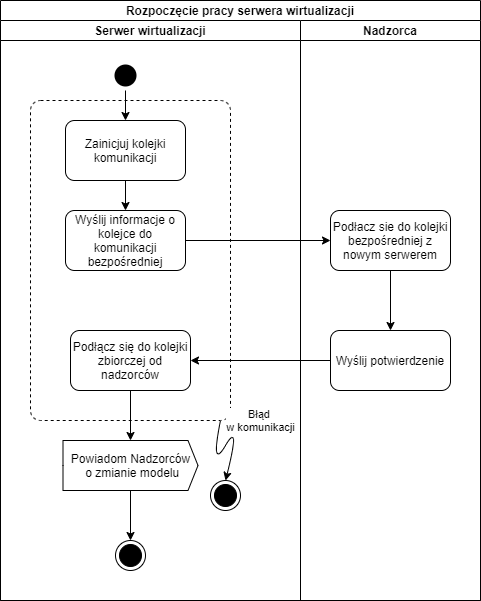
\includegraphics[width=\screenswidth]{activity_diagrams/serwer_start.png}
	
	\vskip-1.5ex
	
	\caption{Diagram aktywności dla rozpoczęcia pracy serwera wirtualizacji}
	\label{start_virtsrv}
\end{figure}

Serwer wirtualizacji bez działającego nadzorcy nie będzie w stanie obsługiwać użytkowników.
Oznacza to, że jeśli przy starcie wystarczająco wiele razy nie wykryje brokera wiadomości
lub nadzorcy po drugiej stronie kolejek\footnote{\href{https://www.rabbitmq.com/confirms.html}{Nadzorcy po drugiej stronie wspólnej kolejki mogą zostać wykryci poprzez mechanizm potwierdzenia wykonania zadania}} to się wyłączy.
Jeżeli jednak nadzorca będzie po drugiej stronie to serwer podłączy się do kolejek \hyperref[external-modules:broker:queue-virtsrv]{wspólnych kolejek} 
oraz przekaże informacje nadzorcom o \hyperref[external-modules:broker:queue-exclusive]{kolejce bezpośredniej}.
Gdy komunikacja będzie ustanowiona bezwarunkowo wyśle stan swojego modelu do nadzorców.

\pagebreak
\end{document}